\documentclass[tikz]{standalone}

\usepackage{amsmath} % for \text
\usepackage{xfrac} % for \myfrac
\usepackage{bm} % for \bm
\usetikzlibrary{calc}
\usetikzlibrary{positioning}
\usetikzlibrary{decorations.pathreplacing,decorations.markings}
\usetikzlibrary{patterns} % 加载 patterns 库
\usepackage{comment}


\colorlet{myred}{red!80!black}
\colorlet{myblue}{blue!80!black}
\colorlet{mygreen}{green!60!black}
\colorlet{myorange}{orange!70!red!60!black}
\colorlet{mydarkred}{red!30!black}
\colorlet{mydarkblue}{blue!40!black}
\colorlet{mydarkgreen}{green!30!black}
\colorlet{myred2}{red!50!white}

\colorlet{mylightblue}{blue!60!cyan!80!black!15}
\colorlet{mypurple}{blue!50!red!70}
\colorlet{gaugecol}{red!90!black!70} % Wiki red
\colorlet{leptoncol}{green!80!black!70} % Wiki green
\colorlet{quarkcol}{blue!85!cyan!95!black!55} % Wiki purple
\colorlet{quarkred}{red!98!black!55} % quark red
\colorlet{quarkblue}{blue!85!cyan!98!black!55} % quark blue
\colorlet{quarkgreen}{green!95!black!55} % quark green
\colorlet{gluoncyan}{cyan!100!black!55} % gluon cyan
\colorlet{gluongreen}{green!75!blue!95!black!70} % gluon green
\colorlet{gluonyellow}{yellow!98!black!55} % gluon yellow
\colorlet{gluonorange}{orange!100!black!65} % gluon orange
\colorlet{gluonmagenta}{magenta!100!black!70} % gluon magenta
\colorlet{scalarcol}{yellow!70!orange!98!black}
\colorlet{tensorcol}{blue!50!red!70} % Wiki light blue
\colorlet{groupcol}{orange!15}

\tikzset{
    mynode/.style={
        circle,        % 形状为圆形
        fill=black,    % 填充颜色为黑色
        inner sep=0.4, % 点的大小
        draw           % 添加边框
    }
}


\begin{document}

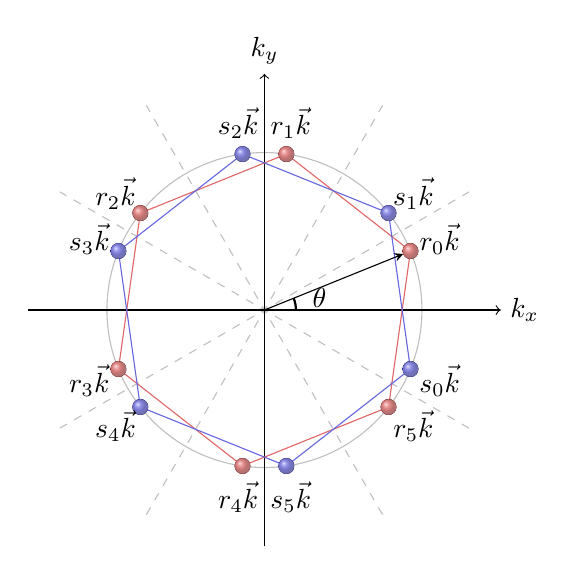
\begin{tikzpicture}[x=2cm, y=2cm]

    \def\RR{1.5}
    \def\N{6}
    \def\th{22}
    \draw[black!25] (0,0) circle (1);

    \foreach \m in {0,...,\numexpr\N-1\relax}{
        % 计算当前点的坐标
        \pgfmathsetmacro{\x}{\RR*cos(360/\N/2*\m)}
        \pgfmathsetmacro{\y}{\RR*sin(360/\N/2*\m)}
        \draw[black!25, dashed] (-\x, -\y) -- (\x, \y);          
    }

% 绘制 x 轴和 y 轴
    \draw[->] (-\RR, 0) -- (\RR, 0) node[right] {$k_x$}; % x 轴
    \draw[->] (0, -\RR) -- (0, \RR) node[above] {$k_y$}; % y 轴
    % 保存第一个点的坐标,用于闭合多边形
    \coordinate (start) at ({cos(360/\N*0 + \th)},{sin(360/\N*0 + \th)});
    
    % 循环绘制点和连接线
    \foreach \m in {0,...,\numexpr\N-1\relax}{
        % 计算当前点的坐标
        \pgfmathsetmacro{\x}{cos(360/\N*\m + \th)}
        \pgfmathsetmacro{\y}{sin(360/\N*\m + \th)}
        
        % 保存点坐标
        \coordinate (current) at (\x,\y);     
        % 连接当前点到下一个点
        \ifnum\m>0
            \draw[myred!60] (prev) -- (current); % 连接上一个点到当前点
        \fi      
        % 更新上一个点
        \coordinate (prev) at (\x,\y);      
    }

    \draw[myred!60] (prev) -- (start);

    \foreach \m in {0,...,\numexpr\N-1\relax}{
        % 计算当前点的坐标
        \pgfmathsetmacro{\x}{cos(360/\N*\m + \th)}
        \pgfmathsetmacro{\y}{sin(360/\N*\m + \th)}
        
         % 绘制点
        \fill[ball color=myred,scale=1,
      postaction={fill=myred!10,opacity=0.5,
      draw=myred!80!black!90,ultra thin}] (\x,\y) circle (0.05);    
      \node at (1.2*\x, 1.2*\y) {$r_\m \vec{k}$};
      
    }

    \coordinate (start) at ({cos(360/\N*0 + \th)},{sin(360/\N*0 - \th)});

     % 循环绘制点和连接线
    \foreach \m in {0,...,\numexpr\N-1\relax}{
        % 计算当前点的坐标
        \pgfmathsetmacro{\x}{cos(360/\N*\m - \th)}
        \pgfmathsetmacro{\y}{sin(360/\N*\m - \th)}
        
        % 保存点坐标
        \coordinate (current) at (\x,\y);
        
        % 连接当前点到下一个点
        \ifnum\m>0
            \draw[myblue!60] (prev) -- (current); % 连接上一个点到当前点
        \fi
       
        % 更新上一个点
        \coordinate (prev) at (\x,\y);
      
    }

    \draw[myblue!60] (prev) -- (start);

    \foreach \m in {0,...,\numexpr\N-1\relax}{
        % 计算当前点的坐标
        \pgfmathsetmacro{\x}{cos(360/\N*\m - \th)}
        \pgfmathsetmacro{\y}{sin(360/\N*\m - \th)}
        
        % 绘制点
        \fill[ball color=myblue,scale=1,
      postaction={fill=myblue!10,opacity=0.5,
      draw=myblue!80!black!90,ultra thin}] (\x,\y) circle (0.05);        
       \node at (1.2*\x, 1.2*\y) {$s_\m \vec{k}$};
    }
  
    %\fill[ball color=myred,scale=1,scale=1, 
    %  postaction={fill=myred!80,opacity=0.6,
    %  draw=myred!50!black!90,thin}] (0,0)  circle(1); % 经典红色球
    %\fill[ball color=myred, shading=ball] (2.5,0) circle (1); % 蓝色球
    %\fill[ball color=mygreen, shading=ball] (5,0) circle (1); % 绿色球
    
    \pgfmathsetmacro{\x}{cos(\th)}
    \pgfmathsetmacro{\y}{sin(\th)}

    \coordinate (O) at (0, 0); % 角的顶点
    \coordinate (A) at (0.95*\x, 0.95*\y); % 第一个边的端点
    \draw[-stealth] (O) -- (A);
\draw[thick] (0.2,0) arc[start angle=0, end angle=\th, radius=0.2];
\node at (0.35,0.075) {$\theta$};

\end{tikzpicture}


\begin{comment}

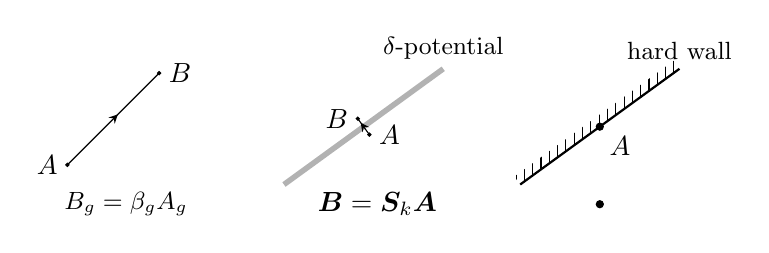
\begin{tikzpicture}[x=2.5cm, y=2.5cm]

\def\th{45}
\def\thth{36}
\def\shift{1.2}
\def\shiftshift{2.4}
\def\De{0.05}
\def\Dy{-0.1}
% 定义点
\coordinate (P1) at (0.1, 0.1);

\pgfmathsetmacro{\x}{cos(\th)}
\pgfmathsetmacro{\y}{sin(\th)}
\coordinate (P2) at (0.8*\x, 0.8*\y);

\pgfmathsetmacro{\x}{0.5*(0.1 + 0.8*cos(\th))}
\pgfmathsetmacro{\y}{\Dy}
\coordinate (P01) at (\x,\y);

\pgfmathsetmacro{\x}{\shift}
\pgfmathsetmacro{\y}{0}
\coordinate (P3) at (\x, \y);

\pgfmathsetmacro{\x}{cos(\thth)+\shift}
\pgfmathsetmacro{\y}{sin(\thth)}
\coordinate (P4) at (\x, \y);

\pgfmathsetmacro{\x}{cos(\thth)/2-\De*cos(\thth+90)+\shift}
\pgfmathsetmacro{\y}{sin(\thth)/2-\De*sin(\thth+90)}
\coordinate (P5) at (\x, \y);

\pgfmathsetmacro{\x}{cos(\thth)/2+\De*cos(\thth+90)+\shift}
\pgfmathsetmacro{\y}{sin(\thth)/2+\De*sin(\thth+90)}
\coordinate (P6) at (\x, \y);

\pgfmathsetmacro{\x}{0.5*(0.0 + 1.0*cos(\thth)) + \shift}
\pgfmathsetmacro{\y}{\Dy}
\coordinate (P02) at (\x,\y);

\pgfmathsetmacro{\x}{\shiftshift}
\pgfmathsetmacro{\y}{0}
\coordinate (P7) at (\x, \y);

\pgfmathsetmacro{\x}{cos(\thth)+\shiftshift}
\pgfmathsetmacro{\y}{sin(\thth)}
\coordinate (P8) at (\x, \y);

\pgfmathsetmacro{\x}{cos(\thth)+\De*cos(\thth+90)+\shiftshift}
\pgfmathsetmacro{\y}{sin(\thth)+\De*sin(\thth+90)}
\coordinate (P9) at (\x, \y);

\pgfmathsetmacro{\x}{\De*cos(\thth+90)+\shiftshift}
\pgfmathsetmacro{\y}{\De*sin(\thth+90)}
\coordinate (P10) at (\x, \y);

\pgfmathsetmacro{\x}{cos(\thth)/2+\shiftshift}
\pgfmathsetmacro{\y}{sin(\thth)/2}
\coordinate (P11) at (\x, \y);

\pgfmathsetmacro{\x}{0.5*(0.0 + 1.0*cos(\thth)) + \shiftshift}
\pgfmathsetmacro{\y}{\Dy}
\coordinate (P03) at (\x,\y);

\node[mynode] at (P1) {};
\node[left] at (P1) {$A$};
\node[mynode] at (P2) {};
\node[right] at (P2) {$B$};
\draw[postaction={decorate}, 
      decoration={markings, mark=at position 0.55 with {\arrow{stealth}}}] (P1) -- (P2);

\draw[gray!60, line width=2.0] (P3) -- (P4);
\node[mynode] at (P5) {};
\node[above] at (P4) {\small $\delta$-potential};
\node[right] at (P5) {$A$};
\node[mynode] at (P6) {};
\node[left] at (P6) {$B$};
\draw[postaction={decorate}, 
      decoration={markings, mark=at position 0.75 with {\arrow{stealth}}}] (P5) -- (P6);

\fill[pattern=vertical lines, pattern color=black] (P7) -- (P8) -- (P9) -- (P10) -- cycle;
\draw[black, thick] (P7) -- (P8);

\node[circle,        % 形状为圆形
        fill=black,    % 填充颜色为黑色
        inner sep=0.9, % 点的大小
        draw   ] at (P11) {};
\node[below right] at (P11) {$A$};
\node[above] at (P8) {\small hard wall};

\node[] at (P01) {\small $\quad B_g=\beta_gA_g$};
\node[] at (P02) {$\quad \bm{B}=\bm{S}_k\bm{A}$};
\node[circle,        % 形状为圆形
        fill=black,    % 填充颜色为黑色
        inner sep=0.9, % 点的大小
        draw   ] at (P03) {};
 
\end{tikzpicture}
\end{comment}

\end{document}